\documentclass{article}
\usepackage[utf8]{inputenc}
\usepackage{mathrsfs}
\usepackage{tikz}
\usepackage{amssymb}
\usepackage{amsthm}
\usepackage{graphicx} % Required for inserting images
\usepackage{amsmath}
\usepackage{MnSymbol}
\usepackage{geometry}
\usepackage{physics}
\usepackage{verbatim}
\usepackage{enumerate}
\allowdisplaybreaks
\newcommand\numeq[1]%
  {\stackrel{\scriptscriptstyle(\mkern-1.5mu#1\mkern-1.5mu)}{=}}
\newcommand\numleq[1]
  {\stackrel{\scriptscriptstyle(\mkern-1.5mu#1\mkern-1.5mu)}{\leq}}
\newcommand\numgeq[1]
  {\stackrel{\scriptscriptstyle(\mkern-1.5mu#1\mkern-1.5mu)}{\geq}}



\title{Math 132H Homework 6}
\author{Tom Slavonia}
\date{\today}

\begin{document}
\maketitle

\section*{1.}
\begin{proof}
We begin by noting that earlier in this course we defined 
\[
 \sin(\pi z) = \pi z - \frac{(\pi z)^3}{3!} + \frac{(\pi z)^5}{5!} + O(z^7)  
\]and thus through our previous homework
\[
 \frac{(\pi z)^2}{\sin(\pi z)^2 } = \left( \frac{\pi z}{\pi z - \frac{(\pi z)^3}{3!} + \frac{(\pi z)^5}{5!} + O(z^7)} \right)^2 = \left( \frac{1}{1 - \frac{(\pi z)^2}{3!} + \frac{(\pi z)^4}{5!}+ O(z^7) }\right)^2 =  \frac{1}{1 - \frac{(\pi z)^2}{3} + \frac{( \pi z)^4}{60} + \frac{(\pi z)^4}{36} + O(z^6)} 
\]
\[
 = \frac{1}{1 - \left(\frac{(\pi z)^2}{3} - \frac{2( \pi z)^4}{45} + O(z^6) \right)} 
\]
and for $z$ close to $0$ (actually for any $|z| < 1$) we have that as the $O(z^6)$ term gets very small
\[
  \frac{(\pi z)^2}{\sin(\pi z)^2 } =\frac{1}{1 - \left(\frac{(\pi z)^2}{3} - \frac{2( \pi z)^4}{45} + O(z^6) \right)} = \sum\limits_{n = 0}^{\infty} \left(\frac{(\pi z)^2}{3} - \frac{2( \pi z)^4}{45} + O(z^6) \right)^n.
\]
It is not easily seem that the coefficient for $z^2$ is $\frac{\pi^2}{3}$ and the coefficient for $z^4$ is $\frac{2\pi^4}{45}$. Similarly, we manipulate the right side of our original equation:
\begin{align*}
  \sum\limits_{n \in \mathbb{Z}, n \neq 0} \frac{z^2}{n^2 - z^2} &= \sum\limits_{n \in \mathbb{Z}, n \neq = 0} \left(\frac{z}{n} \right)^2 \cdot \frac{1}{\left(1 - \frac{z}{n} \right)^2} \\
  &= \sum\limits_{n \in \mathbb{Z}, n \neq = 0} \left(\frac{z}{n} \right)^2 \cdot \frac{1}{1 - \left(\frac{2z}{n} - \frac{z^2}{n^2}\right)} \\
  &= \sum\limits_{n \in \mathbb{Z}, n \neq = 0} \left(\frac{z}{n} \right)^2\sum\limits_{m = 0}^{\infty} \left(\frac{2z}{n} - \frac{z^2}{n^2} \right)^m \\
  &= \sum\limits_{n \in \mathbb{Z}, n \neq = 0} \left(\frac{z}{n} \right)^2\left(1 + \frac{2z}{n} - \frac{z^2}{n^2} +\frac{4z^2}{n^2} + O(z^3) \right) \\
  &= \sum\limits_{n \in \mathbb{Z}, n \neq = 0} \frac{z^2}{n^2} + \frac{4z^3}{n^3} + \frac{6z^4}{n^4} + O(6).
\end{align*}
With $\frac{\pi^2z^2}{\sin^2(\pi z)}$ begin holomorphic everywhere except the integers it must be that the right and left coefficients match and thus 
\[
 \frac{\pi^2}{3} = \sum\limits_{n = 0}^{\infty}\frac{2}{n^2} \Rightarrow \frac{\pi^2}{6} = \sum\limits_{n = 0}^{\infty} \frac{1}{n^2} 
\]
and 
\[
 \frac{2 \pi^4}{45} = \sum\limits_{n = 0}^{\infty} \frac{4 \pi^4}{n^4} \Rightarrow \frac{\pi^4}{90} = \sum\limits_{n = 0}^{\infty} \frac{1}{n^4}. 
\]
\end{proof}
\section*{10.}

\begin{center}
    

\tikzset{every picture/.style={line width=0.75pt}} %set default line width to 0.75pt        

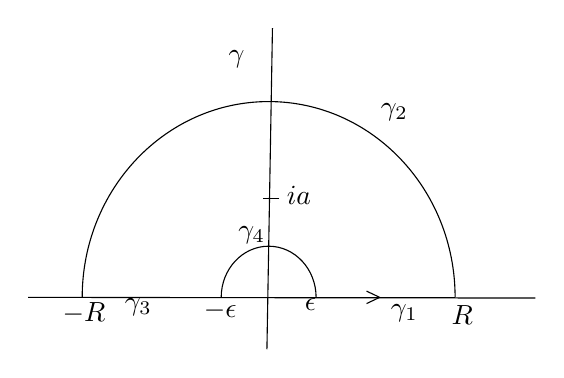
\begin{tikzpicture}[x=0.5pt,y=0.5pt,yscale=-1,xscale=1]
%uncomment if require: \path (0,451); %set diagram left start at 0, and has height of 451

%Shape: Arc [id:dp9648181515346679] 
\draw  [draw opacity=0] (184,243.5) .. controls (184,243.5) and (184,243.5) .. (184,243.5) .. controls (184,243.5) and (184,243.5) .. (184,243.5) .. controls (184,165.35) and (244.33,102) .. (318.75,102) .. controls (393.17,102) and (453.5,165.35) .. (453.5,243.5) -- (318.75,243.5) -- cycle ; \draw   (184,243.5) .. controls (184,243.5) and (184,243.5) .. (184,243.5) .. controls (184,243.5) and (184,243.5) .. (184,243.5) .. controls (184,165.35) and (244.33,102) .. (318.75,102) .. controls (393.17,102) and (453.5,165.35) .. (453.5,243.5) ;  
%Shape: Arc [id:dp6113275985158917] 
\draw  [draw opacity=0] (284.46,243.5) .. controls (284.46,243.5) and (284.46,243.5) .. (284.46,243.5) .. controls (284.46,243.5) and (284.46,243.5) .. (284.46,243.5) .. controls (284.46,223.08) and (299.81,206.53) .. (318.75,206.53) .. controls (337.69,206.53) and (353.04,223.08) .. (353.04,243.5) -- (318.75,243.5) -- cycle ; \draw   (284.46,243.5) .. controls (284.46,243.5) and (284.46,243.5) .. (284.46,243.5) .. controls (284.46,243.5) and (284.46,243.5) .. (284.46,243.5) .. controls (284.46,223.08) and (299.81,206.53) .. (318.75,206.53) .. controls (337.69,206.53) and (353.04,223.08) .. (353.04,243.5) ;  
%Straight Lines [id:da17167570781740116] 
\draw    (184,243.5) -- (284.46,243.5) ;
%Straight Lines [id:da10751477565070289] 
\draw    (353.04,243.5) -- (453.5,243.5) ;
%Straight Lines [id:da9733644721386747] 
\draw    (145,243.5) -- (511.5,244) ;
\draw   (389.5,239) -- (399,243.5) -- (389.5,248) ;
%Straight Lines [id:da7761560722072005] 
\draw    (317.5,281) -- (321.5,49) ;
%Straight Lines [id:da2763300965420783] 
\draw    (326.5,172) -- (314.5,172) ;

% Text Node
\draw (270,244.4) node [anchor=north west][inner sep=0.75pt]    {$-\epsilon $};
% Text Node
\draw (343,242.4) node [anchor=north west][inner sep=0.75pt]    {$\epsilon $};
% Text Node
\draw (330,161.4) node [anchor=north west][inner sep=0.75pt]    {$ia$};
% Text Node
\draw (168,245.4) node [anchor=north west][inner sep=0.75pt]    {$-R$};
% Text Node
\draw (449,247.4) node [anchor=north west][inner sep=0.75pt]    {$R$};
% Text Node
\draw (405.27,246.9) node [anchor=north west][inner sep=0.75pt]    {$\gamma _{1}$};
% Text Node
\draw (398,101.4) node [anchor=north west][inner sep=0.75pt]    {$\gamma _{2}$};
% Text Node
\draw (213,242.4) node [anchor=north west][inner sep=0.75pt]    {$\gamma _{3}$};
% Text Node
\draw (295,190.4) node [anchor=north west][inner sep=0.75pt]    {$\gamma _{4}$};
% Text Node
\draw (288,63.4) node [anchor=north west][inner sep=0.75pt]    {$\gamma $};


\end{tikzpicture}
\end{center}
\begin{proof}
    Consider the countour as above. Take $f(z) = \frac{\log^2(z)}{z^2 + a^2}$ and we have 
    \[
    \int_{\gamma}f(z) dz = \int_{\gamma_1}f(z) dz + \int_{\gamma_2}f(z)dz - \int_{\gamma_3} f(z) dz - \int_{\gamma_4}f(z)dz = \int_{\epsilon}^R f(x)dx + \int_{\gamma_2} f(z)dz + \int_{-R}^{-\epsilon} f(x) dx   - \int_{\gamma_4}f(z) dz.
    \] 
    The princial branch for the logarithm as $\log(z) = \log(R) + i \theta$ for $z = Re^{i \theta}$ but to avoid discontinuities along that line take the branch cut from $-\frac{\pi}{2}$ to $\frac{3 \pi}{2}$ which is the negative imaginary access on which our contour takes no values. 
    By the residue formula for toy contours, we have that the integral around the toy contours is equal to the sum of the residues multiplied by $2\pi i$. We can begin by finding the poles of $f(z)$ by 
    \[
    \frac{1}{f(z)} = \frac{z^2 + a^2}{\log^2(z)} = 0    
    \]
    so our poles occur when 
    \[
    z^2 + a^2 = 0    
    \]
    and we have that 
    \[
    z^2 + a^2 = (z + ia)(z -ia ) = 0     
    \]
    and thus we obtain the poles $z = ia, -ia$. But, we are only considering the upper-indented semicircle, and thus $z = ia$ is the only pole within the contour. Writing 
    \[
    f(z) = (z - ia)^{-1} \frac{\log^2(z)}{z + ia}    
    \]
    we are able to identify that the pole $ia$ has order $1$ as $\frac{\log(z)}{z + ia}$ is holomorphic at $z = ia$. Calculating the pole's residue, we then have
    \[
       \text{res}_{ia}f = \lim\limits_{z \to ia}(z - ia) \frac{\log^2(z)}{(z - ia)(z + ia)} =  \frac{\log^2(ia)}{2ia}  = \frac{(\log(a) + i\pi)^2}{2ai}
    \]
    with $\theta = \frac{\pi}{2}$ as $ia$ lies on the imaginary axis. We will now show the decay of some of our line integrals. For instance,  
    \begin{align*}
        \left|\int_{\gamma_2}f(z) dz \right| &= \left|\int_{0}^{\pi} \frac{(\log(R) + i \theta)^2}{\left(Re^{i \theta}\right) + a^2} Rie^{i \theta}d \theta \right| \\
        &\leq \int_{0}^{\pi}\frac{|\log(R) + i \theta|^2}{R^2 - a^2}Rd \theta \\
        & =\frac{R}{R^2 - a^2} \int_0^{\pi} (\log(R)+ \theta d \theta)^2\\
        &\leq \frac{R\log(R) + 2R
      \log(R)\frac{3 \pi}{2} + R\left(\frac{3 \pi}{2}\right)^2}{R^2 - a^2}.
    \end{align*}
    With L'Hopital's rule we have that 
    \[
    \lim\limits_{R \to \infty} \frac{R \log(R)}{R^2 - a^2} = \lim\limits_{R \to \infty} \frac{\log(R)}{2R} = \lim\limits_{R \to \infty} \frac{1}{2R} = 0.    
    \]
    and thus
    \[
    \lim\limits_{R \to \infty} \left|\int_{\gamma_3}f(z)dz \right| = 0.    
    \]
    A similar bound can be placed on the integral around the indent: 
    \begin{align*}
        \left|\int_{\gamma_4}f(z) dz \right| & = \left|\int_{\pi}^0 \frac{(\log\left(\epsilon\right) + i \theta)^2}{\left(\epsilon e^{i \theta}\right)^2 + a^2} \epsilon i e^{i \theta } d \theta \right| \\
        &\leq \int_{\pi}^0 \frac{(\log(\epsilon) + \theta)^2}{\epsilon^2 - a^2}\epsilon d \theta \\
        &\leq \epsilon \pi\frac{\left(\log(\epsilon) + \frac{3\pi}{2}\right)^2}{\epsilon^2 - a^2}\\
        &= \epsilon \pi\frac{\log^2(\epsilon) + 3 \pi \log(\epsilon) + \frac{9\pi}{4}}{\epsilon^2 - a^2}
    \end{align*}
    The limit 
    \[
    \lim\limits_{\epsilon \to 0} \frac{\epsilon \log(\epsilon)}{\epsilon^2 - a^2} = \lim\limits_{\epsilon \to 0} \frac{\epsilon \log(\epsilon)}{-a^2}
    \]
    requires more careful consideration. Use the substitution $\epsilon = e^{-u}$ and we know review
    \[
      \lim\limits_{\epsilon \to 0} \epsilon \log(\epsilon) = \lim\limits_{u \to \infty} -u e^{-u} = 0.   
    \]
    Thus, 
    \[
      \lim\limits_{\epsilon \to 0}\left|\int_{\gamma_4}f(z) dz \right| = 0.  
    \]
    Now we inspect 
    \[
    \int_{\epsilon}^R \frac{\log^2(z)}{z^2 + a^2}dz = \int_{\epsilon}^R \frac{\left(\log(x) + i\frac{ \pi}{2}\right)^2}{x^2 + a^2}dx  \text{ and } \int_{-R}^{\epsilon} \frac{\log^2(z)}{z^2 + a^2}dx = \int_{-R}^{-\epsilon} \frac{\left(\log(x) + i \frac{3 \pi }{2}\right)^2}{x^2 + a^2} dx =  \int_{\epsilon}^R\frac{\left(\log(x) + i \frac{3 \pi }{2}\right)^2}{x^2 + a^2} dx
    \]
    as $R \to \infty$ and $\epsilon \to 0$ and a change of variables $x = -x$ in the second integral. By the residue theorem we have 
    \[
      \lim\limits_{\epsilon \to 0} \lim\limits_{R \to \infty} \int_{\epsilon}^R \frac{\left(\log(x) + i\frac{ \pi}{2}\right)^2}{x^2 + a^2}dx + \int_{\epsilon}^{R} \frac{\left(\log(x) + i \frac{3 \pi }{2}\right)^2}{x^2 + a^2} dx\]\[ = \int_{0}^{\infty} \frac{\left(\log(x) + i\frac{ \pi}{2}\right)^2}{x^2 + a^2}dx + \int_{0}^{\infty} \frac{\left(\log(x) + i \frac{3 \pi }{2}\right)^2}{x^2 + a^2} dx = 2 \pi i \left( \frac{(\log(a) + i\pi)^2}{2ai} \right).\]
      
      After some extensive simplifying we get the desired result
      \[
      \int_0^{\infty} \frac{\log(x)}{x^2 + a^2} dx = \frac{\pi \log(a)}{2a}. 
      \]

    


\end{proof}

\section*{11.}
\begin{proof}
 With $|a| < 1$, then, if we parametrize $z = ae^{i \theta}$ then
 \[
 \int_0^{2 \pi}\log\left|1 - ae^{i \theta}\right|d \theta = \int_{|z| = a}\frac{\log|1 - z|}{iz}dz 
 \]
 and we can see that the only pole of $f(z) = \frac{\log|1 - z|}{iz}$ is then $z = 0$ of order $1$. Our residue calculation then becomes
 \[
 \text{res}_{z_0 = 0}f = \lim\limits_{z \to 0} (z - 0) \frac{\log|1 - z|}{iz} = \lim\limits_{z \to 0} \frac{\log|1 - z|}{i} = \frac{\log(1)}{i} = 0.
 \]
 Thus, the integral 
 \[
 \int_0^{2 \pi } \log\left|1 - ae^{i \theta}\right| d\theta = 0 
 \]
 when $|a| < 1$. 

 Now suppose $|a| \leq 1$. Use the drawing below and for $f(z) = \frac{\log|1 - z|}{iz}$ decompose the integral into 
 \[
 \int_{\gamma_{\epsilon}}f(z)dz - \int_{\gamma}f(z)dz = \int_{\gamma_C} f(z)dz. 
 \]Beginning by inspecting 
 \[
 \int_{\gamma_C}f(z)dz 
 \] we have 
 \begin{align*}
 \left|\int_{\gamma_C} f(z) dz \right| &\leq \int_{\pi}^0 \frac{\log|1 - z|}{|z|}dz \\
 &\leq \epsilon \max\limits_{z \in C}|\log( 1- z)| \\
 &\leq \epsilon \log(1 - 1 + \epsilon)\\
 &= \epsilon \log(\epsilon) \xrightarrow[\epsilon \to 0]{} 0 \text{ (we proved this in the previous question)}.
 \end{align*}
Note, that through our previous work we have that 
\[
 \int_{\gamma}f(z) dz = 0. 
\]
Hence, we get the result 
\[
 \lim\limits_{\epsilon \to 0} \int_{\gamma_{\epsilon}} f(z)dz - \int_{\gamma}f(z)dz = \lim\limits_{\epsilon \to 0} \int_{\epsilon}^{2 \pi - \epsilon}\log\left|1 - ae^{i \theta}\right|d \theta = \int_0^{2 \pi}\log\left|1 - ae^{i \theta}\right|d \theta = 0.
\]
\begin{center}
  

\tikzset{every picture/.style={line width=0.75pt}} %set default line width to 0.75pt        

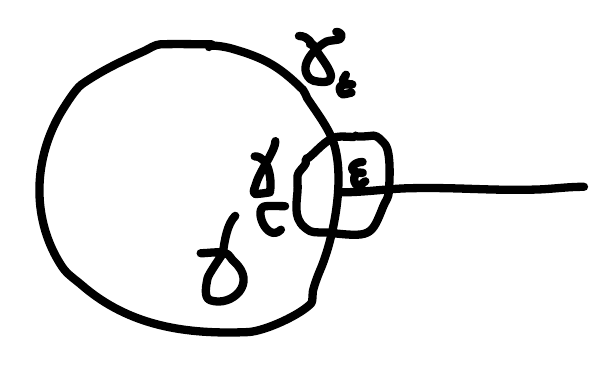
\begin{tikzpicture}[x=0.5pt,y=0.5pt,yscale=-1,xscale=1]
%uncomment if require: \path (0,451); %set diagram left start at 0, and has height of 451

%Shape: Free Drawing [id:dp11021507652696605] 
\draw  [line width=3] [line join = round][line cap = round] (342.5,148) .. controls (330.17,148) and (317.83,147.68) .. (305.5,148) .. controls (301.36,148.11) and (297.18,151.36) .. (293.5,153) .. controls (277.61,160.06) and (263.25,166.74) .. (248.5,177) .. controls (243.37,180.57) and (233.66,196.95) .. (232.5,199) .. controls (213.08,233.21) and (212.47,275.96) .. (234.5,309) .. controls (238.08,314.37) and (243.73,317.86) .. (248.5,322) .. controls (282.98,351.88) and (324.1,357.81) .. (368.5,356) .. controls (380.81,355.5) and (407.33,343.2) .. (414.5,335) .. controls (415.51,333.85) and (415.32,328.1) .. (415.5,327) .. controls (416.19,322.85) and (419.59,314.09) .. (420.5,312) .. controls (431.34,287.22) and (440.36,238.9) .. (428.5,214) .. controls (423.93,204.4) and (417.4,195.85) .. (411.5,187) .. controls (410.26,185.14) and (410.08,182.58) .. (408.5,181) .. controls (390.57,163.07) and (379.48,157.57) .. (356.5,151) .. controls (352.07,149.73) and (340.5,147.8) .. (340.5,150) ;
%Shape: Free Drawing [id:dp7579035278598978] 
\draw  [line width=3] [line join = round][line cap = round] (445.5,215) .. controls (441.17,215) and (436.77,214.29) .. (432.5,215) .. controls (425.51,216.16) and (417.66,225.99) .. (412.5,230) .. controls (411.91,230.46) and (410.68,230.28) .. (410.5,231) .. controls (410.26,231.97) and (410.87,233.07) .. (410.5,234) .. controls (409.39,236.76) and (404.75,239.98) .. (404.5,243) .. controls (404.2,246.65) and (404.8,250.35) .. (404.5,254) .. controls (403.46,266.49) and (401.33,276.24) .. (413.5,283) .. controls (416.14,284.46) and (423.83,283.81) .. (425.5,284) .. controls (457.84,287.59) and (457.64,287.14) .. (466.5,265) .. controls (468.33,260.43) and (470.14,259.83) .. (470.5,254) .. controls (470.63,251.93) and (472.82,225.98) .. (467.5,220) .. controls (465.29,217.51) and (462.81,214.37) .. (459.5,214) .. controls (459.09,213.96) and (446.5,215.59) .. (446.5,214) ;
%Shape: Free Drawing [id:dp08610030762496135] 
\draw  [line width=3] [line join = round][line cap = round] (435.5,255) .. controls (453.26,255) and (469.31,252.32) .. (486.5,252) .. controls (522.44,251.32) and (542,253.86) .. (576.5,253) .. controls (588.46,252.7) and (598.43,251) .. (611.5,251) ;
%Shape: Free Drawing [id:dp015772714944722654] 
\draw  [line width=3] [line join = round][line cap = round] (451.5,233) .. controls (443.89,233) and (439.16,241) .. (451.5,241) .. controls (452.83,241) and (448.69,240.4) .. (447.5,241) .. controls (445.1,242.2) and (444.78,246.94) .. (446.5,249) .. controls (449.67,252.81) and (452.05,247) .. (453.5,247) ;
%Shape: Free Drawing [id:dp7211492822545107] 
\draw  [line width=3] [line join = round][line cap = round] (413.5,148) .. controls (417.53,148) and (416.73,150.17) .. (418.5,153) .. controls (422.96,160.14) and (438.51,177.72) .. (419.5,175) .. controls (417.41,174.7) and (414.99,174.49) .. (413.5,173) .. controls (403.33,162.83) and (419.4,149.05) .. (425.5,146) .. controls (427.15,145.18) and (434.73,145.03) .. (435.5,144) .. controls (438.04,140.62) and (434.2,139) .. (432.5,139) ;
%Shape: Free Drawing [id:dp47820889520811183] 
\draw  [line width=3] [line join = round][line cap = round] (439.5,170) .. controls (439.5,172.36) and (436.58,172.24) .. (437.5,175) .. controls (438.23,177.18) and (446.88,177) .. (443.5,177) .. controls (440.67,177) and (431.19,176.04) .. (436.5,184) .. controls (437.03,184.8) and (442.62,183) .. (443.5,183) ;
%Shape: Free Drawing [id:dp8922910343742905] 
\draw  [line width=3] [line join = round][line cap = round] (405.5,142) .. controls (412.62,142) and (414.42,147.38) .. (417.5,152) ;
%Shape: Free Drawing [id:dp029263631228143794] 
\draw  [line width=3] [line join = round][line cap = round] (373.5,229) .. controls (384.51,229) and (386.02,247.89) .. (384.5,255) .. controls (384.5,255.01) and (374.21,256.71) .. (373.5,256) .. controls (371.83,254.33) and (373.93,251.29) .. (374.5,249) .. controls (376.63,240.5) and (388.5,224.93) .. (388.5,218) ;
%Shape: Free Drawing [id:dp012841757285598776] 
\draw  [line width=3] [line join = round][line cap = round] (395.5,265) .. controls (390.83,265) and (386.16,264.69) .. (381.5,265) .. controls (371.83,265.64) and (382.28,292.22) .. (392.5,282) ;
%Shape: Free Drawing [id:dp15801644501928003] 
\draw  [line width=3] [line join = round][line cap = round] (334.5,299) .. controls (340.5,299) and (346.68,297.54) .. (352.5,299) .. controls (355.24,299.69) and (356.37,303.14) .. (358.5,305) .. controls (376.02,320.33) and (357.17,338.22) .. (341.5,333) .. controls (336.4,331.3) and (338.45,322.27) .. (339.5,317) .. controls (340.09,314.07) and (350.41,299.62) .. (350.5,299) .. controls (351.79,289.99) and (353.49,278.01) .. (359.5,272) ;




\end{tikzpicture}
\end{center}
\end{proof}

\section*{4.}
\begin{proof}
  With $f^n$ holomorphic for all $n$ there exists 
  \[
  \lim\limits_{h \to 0} \frac{f^n(w + h) - f^n(w)}{h}.  
  \]
  Let this limit equal $L$. Then, 
  \[
  \lim\limits_{h \to 0} \frac{f(w + h) - f(w)}{h} \cdot \left(\sum\limits_{k = 0}^{n -1}f^{n-k - 1}(w + h)f^k(w) \right)  
  \]
  implies by the continuity of $f$
  \begin{align*}
  \lim\limits_{h \to 0}\frac{f(w + h) - f(w)}{h} &= \lim\limits_{h \to 0}\frac{L}{\left(\sum\limits_{k = 0}^{n -1}f^{n-k - 1}(w + h)f^k(w) \right)} \\
  &= \frac{L}{\sum\limits_{k = 0}^{n - 1}f^{n -k - 1}(w)f^k(w)} \\
  &= \frac{L}{\sum\limits_{k = 0}^{n -1}f^{n-1}(w)} \\
  &= \frac{L}{nf^{n - 1}(w)}. 
  \end{align*}
  and we have by the continuity of $f$ that $f^{n -1}(w)$ is bounded and thus that $f$ at any singularity would be bounded. Thus, the singularity would be removable and $f$ could be defined to be holomorphic on $\Omega$.    
\end{proof}

\section*{18.}
\begin{proof}
  Suppose $f$ is holomorphic in an open set that contains the closure of a disc $D$. Suppose $C$ is the boundary circle of the disc. Note, that a circle has the same start and end points. We then have
  \[
  \frac{1}{2 \pi i }\int_C \frac{f(\zeta)}{\zeta - z_0}d \zeta = \frac{1}{2 \pi i } \int_C \frac{f(\zeta) - f(z_0)}{\zeta - z_0} d \zeta + \frac{f(z_0)}{2 \pi i} \int_C \frac{1}{\zeta - z_0}d\zeta .  
  \]
  Using the hint, we deform the circle $C$ continuously into the circle $C_r$ the circle of radius $r$ centered around $z_0$. Since $f$ is holomorphic in the open set that contains the disc, we have by theorem 5.1 
  \[
    \frac{1}{2 \pi i }\int_C \frac{f(\zeta)}{\zeta - z_0}d \zeta = \frac{1}{2 \pi i } \int_C \frac{f(\zeta) - f(z_0)}{\zeta - z_0} d \zeta + \frac{f(z_0)}{2 \pi i} \int_C \frac{1}{\zeta - z_0}d\zeta = \frac{1}{2 \pi i } \int_{C_r} \frac{f(\zeta) - f(z_0)}{\zeta - z_0} d \zeta + \frac{f(z_0)}{2 \pi i} \int_{C_r} \frac{1}{\zeta - z_0}d\zeta.
  \]
  We've previously shown, that since the circle $C_r$ is centered around $z_0$, we have
  \[
  \int_{C_r} \frac{1}{\zeta - z_0} = 2 \pi i.  
  \]
  Employing the hint that $\frac{f(\zeta) - z}{\zeta - z}$ is bounded, suppose for some $|M| > 0$, then we have that
  \[
    \left|\frac{1}{2 \pi i } \int_{C_r} \frac{f(\zeta) - f(z_0)}{\zeta - z_0}d \zeta \right| \leq \frac{2Mr}{2 \pi} \xrightarrow[r \to 0]{} 0.
  \]
  Combining our results we have that as $r \to 0$.
  \[
  \frac{1}{2 \pi i } \int_C \frac{f(\zeta)}{\zeta - z_0} d \zeta = \frac{f(z_0)}{2 \pi i} \cdot 2 \pi i = f(z_0).   
  \]
\end{proof}

\section*{21.}
\subsection*{a.}
\begin{proof}
  Suppose $\gamma_1, \gamma_2 \in \Omega$ are two curves with the same endpoints $\alpha$ and $\beta$. By the convexity of $\Omega$ there exists a straight line $\gamma_s \in  \Omega$ such that $\gamma_s(a) = \alpha$ and $\gamma_s(b) = \beta$ and define 
  \[
  F(s, t) = s\gamma_2(t) + (1 - s) \gamma_1(t).
  \]
  with $s \in [0, 1]$ and $t \in [a, b]$. 
  This is the line between the two curves at every point, so it is always in the set $\Omega$ by convexity. We have that $F(s, 0) = \alpha$, $F(s, 1) = \beta$, $F(0, t) = \gamma_1(t)$, and $F(1, t) = \gamma_2(t)$ and thus the properties for the curves being homotopic are satisfied and we chose arbitrary curves with the same endpoint in $\Omega$, thus $\Omega$ is simply connected. 
\end{proof}
\subsection*{b.}
\begin{proof}

  

  Suppose $\gamma_1(t)$ and $\gamma_2(t)$ are defined just as they were in the first part of the problem. 
  Define a homotopy
  \[
  \gamma_s(t) = \begin{cases}
    2 s \gamma_1(t) (1 - 2s)z_0, \ s \in \left[0, \frac{1}{2} \right] \\
    2(s - 1)z_0 + (2s - 1)\gamma_2(t), \ s \in\left[\frac{1}{2}, 1 \right].
  \end{cases}  
  \]
  We always have that $\gamma_s(t) \in \Omega$ as we know there exists a line segment from $z_0$ to any point in the set as the set is star-shaped. To verify that this is a homootpy, we have $\gamma_s(a) = \alpha$, $\gamma_s(b) = \beta$, $\gamma_0(t) = \gamma_1(t)$ and $\gamma_1(t) = \gamma_2(t)$. 
  Therefore, we have satisfied all conditions for a homotopy and we have simple connectedness.  
  \subsection*{c.}
  The empty set.  
\end{proof}
\section*{22.}
\begin{proof}
  For the sake of contradiction, suppose that there is a holomorphic function $f$ in the unit disc $\mathbb{D}$ that extends continuously to $\partial \mathbb{D}$ such that $f(z) = \frac{1}{z}$ for $z \in \partial \mathbb{D}$. We've previously found the result that 
  \[
  \int_{|z| = 1} \frac{1}{z} dz = 2 \pi i.   
  \] We have that for a disc of radius $0 < r < 1$ we know $f$ is holomorphic in that disc, so by Cauchy's theorem
  \[
  \int_{D_r}f(z)dz = 0. 
  \]
  $f$ is continuous on the boundary of the circle and note that $\bar{\mathbb{D}} = \partial \mathbb{D} \cup \mathbb{D}$ is closed and bounded in a compact space, then we can use uniform continuity on the closed disc to state
  \[
    0 = \lim\limits_{r \to 1}\int_{z = |r|} f(z)dz = \int_{|z| = 1}f(z) dz = \int_{|z| = 1} f(z) dz = \int_{|z| = 1} \frac{1}{z}dz = 2 \pi i
  \]
  which is a contradiction. 
\end{proof}

\section*{8.}
\begin{proof}
  Begin by noting that \[
  x^4 + 2x^2 - x + 1 = x^4 + x^2 + \left(x - \frac{1}{2}\right)^2 + \frac{3}{4} > 0  
  \]
  \[
  (iz)^4 + (iz)^2 -iz + 1 = z^4 - z^2 -iz + 1 \neq 0
  \]
  so no zeros exist on the real or imaginary line. By the argument principle
  \[
  \frac{1}{2 \pi i }\int_C \frac{4z^3 + 4z - z}{z^4 + z^2 -z + 1} dz = (\text{number of zeros of }f \text{ inside }C) \text{ minus } (\text{ number of poles of } f \text{ inside }C).
  \]
  Let $\gamma_R$ be the first quadrant of the circle contour with boundary of $D_R = \{z = re^{i \theta} : 0 < r < R, 0 < \theta < \frac{\pi}{2} \}$. For the straight line on the real axis from $0$ to $R$ we have $0 \leq x \leq R$, $p(z) \geq \frac{3}{4}$ and $\Delta p(z) = 0$, so $arg(p(z(x))) \equiv 0$. Considering the curve from $z = R$ where $z = Re^{it}$ for $0 \leq t \leq \frac{\pi}{2}$ we have 
  \[
  p(z) = z^4(1 + 2z^{-2} - z^{-3} + z^{-4})  
  \]
  and thus $\Delta_{\gamma_2}p(z) = \Delta_{\gamma_2}z^4 + O(1) \approx 4 \cdot \frac{\pi}{2} + O(1) = 2 \pi + O(1)$ with $O(1) \to 0$ as $R \to \infty$. Now for $\gamma_3$ when $z = it$ for $t$ decreasing from $R$ to $0$, then 
  \[
  p(it) = t^4 - t^2 -it + 1  
  \]
  and thus it must be in the lower half plane as we have $-it$. As $t \to 0$ we get 
  \[
  \lim\limits_{t \to 0} p(it) = 1   
  \]
  and 
  \[
  \Delta_{\gamma_3} p(z) \to 0.  
  \]
  Therefore, $\Delta_{\gamma}arg(p(z)) = 2 \pi + O(1)$. Therefore, for the first quadrant we clearly have no poles of $p(z)$ and thus 
  the number of zeros in the first quadrant is 
  \[
  \frac{1}{2 \pi i}\int_C \frac{p'(z)}{p(z)}dz = \frac{2 \pi }{2 \pi } = 1.  
  \]
  Therefore, there is a zero in every quadrant since every coeffcient is real the zeros come in pairs and we have order $4$ polynomial, so we have a zero in each quadrant. 
\end{proof}
\end{document}